%\documentclass[11pt, oneside]{article}   	% use "amsart" instead of "article" for AMSLaTeX format
%\usepackage{geometry}                		% See geometry.pdf to learn the layout options. There are lots.
%\geometry{letterpaper}                   		% ... or a4paper or a5paper or ... 
%\geometry{landscape}                		% Activate for for rotated page geometry
%\usepackage[parfill]{parskip}    		% Activate to begin paragraphs with an empty line rather than an indent
%\usepackage{graphicx}				% Use pdf, png, jpg, or eps§ with pdflatex; use eps in DVI mode
%								% TeX will automatically convert eps --> pdf in pdflatex		
%\usepackage{amssymb,amsmath}
\newcommand{\sph}[2]{Y^\text{R}_{l_#1 m_#1}(\hat{#2})}

\newcommand{\jl}[1]{j_{l_#1}}
\newcommand{\dk}{\frac{ d^3 \mathbf{k}}{(2 \pi)^3}} 
\newcommand{ \dkv}[1]{\frac{ d^3 \mathbf{k}_{#1}}{(2 \pi)^3}} 
\newcommand{\obs}{\mathcal{O}}

\subsection{Spherical basis functions}
For spherical geometry we use the following basis, composed of the spherical Bessel function and spherical harmonic:
\begin{align} 
\psi_\alpha(r, \theta, \phi) = j_{l_\alpha}(k_\alpha r) Y^\text{R}_{l_\alpha m_\alpha}(\theta, \phi) ~, 
\end{align} 
where $Y^\text{R}_{lm}(\theta, \phi) $ is the real spherical harmonic. The real spherical harmonics are defined as 
\begin{align}
Y^\text{R}_{lm} =
\begin{cases} \frac{i}{\sqrt{2}} \left( Y_{lm}  - (-1)^m Y_{l-1m} \right)& \text{if }  m < 0 \\
Y_{l0} & \text{if } m=0 \\
\frac{1}{\sqrt{2}}\left( Y_{l-m} + (-1)^mY_{lm}\right) & \text{if } m > 0 ~.
\end{cases}
\end{align} 
The bias functions are defined within a ball, with a maximum radius $R_\text{max}$ that corresponds to a redshift larger than any survey redshift.  The $k_\alpha$ are determined by \begin{align}
 j_{l_\alpha}(k_\alpha R_\text{max})=0.
\end{align}
We write a super survey mode as 
\begin{align}
\delta_\alpha& = \frac{1}{N_\alpha}  \int \delta(\mathbf{r}) \jl{\alpha}(k_\alpha r) \sph{\alpha}{r} d^3 \mathbf{r}~. 
\end{align}
The normalization to the super mode is 
\begin{align} 
N_\alpha= \int_0^{R_\text{max}} dr r^2 j_{l_\alpha} (k_\alpha r) j_{l_\alpha} (k_\alpha r) ~.
\end{align} 

\subsubsection{Mean background density in a region}
The mean background density in a region is composed of the super modes:

\begin{align}
\label{bar_delta}
\begin{split} 
\bar{\delta} & = \frac{1}{\text{volume}} \int_{r_1, \theta_1, \phi_1}^{r_2, \theta_2, \phi_2} d^3 \mathbf{x} \delta(\mathbf{x}) \\
& = \displaystyle \sum_\alpha \frac{3}{r_2^3 - r_1^3} \int_{r_1}^ {r_2 }dr ~ r^2 j_{l_\alpha}(k_\alpha r) \delta_\alpha \frac{1}{2\sqrt{\pi} a_{00}} \underbrace{ \int_{\theta_1}^{\theta_2 }\int_{\phi_1}^{\phi_2} d  \theta d \phi ~\sin(\theta)\sph{\alpha}{r}}_{a_{l_\alpha m_\alpha}} ~.
\end{split}
\end{align}
Note that the integral is not over the ball that we define our basis functions in. It is over a survey region or slice of the survey. 


In practice we are interested in derivatives of observables with respect to the $\delta_\alpha$. This is accomplished by chain rule 
\begin{align}
\frac{\partial f}{\partial \delta_\alpha}= \frac{\partial f}{\partial \bar{\delta}} \frac{\partial \bar{\delta}}{\partial \delta_\alpha}~.
\end{align} 
The derivative is computed from Eqn.~\ref{bar_delta}
\begin{align}
\frac{\partial \bar{\delta} }{ \partial \delta_\alpha}=
\frac{3}{r_2^3 - r_1^3} \int_{r_1}^{r_2} dr ~ r^2 j_{l_\alpha}(k_\alpha r)  \frac{1}{2\sqrt{\pi} a_{00}}  \int_{\theta_1}^{\theta_2 } \int_{\phi_1}^{\phi_2} d\theta d \phi ~\sin(\theta)\sph{\alpha}{r}~.
\end{align}

 \begin{figure}[!ht]
 \centering
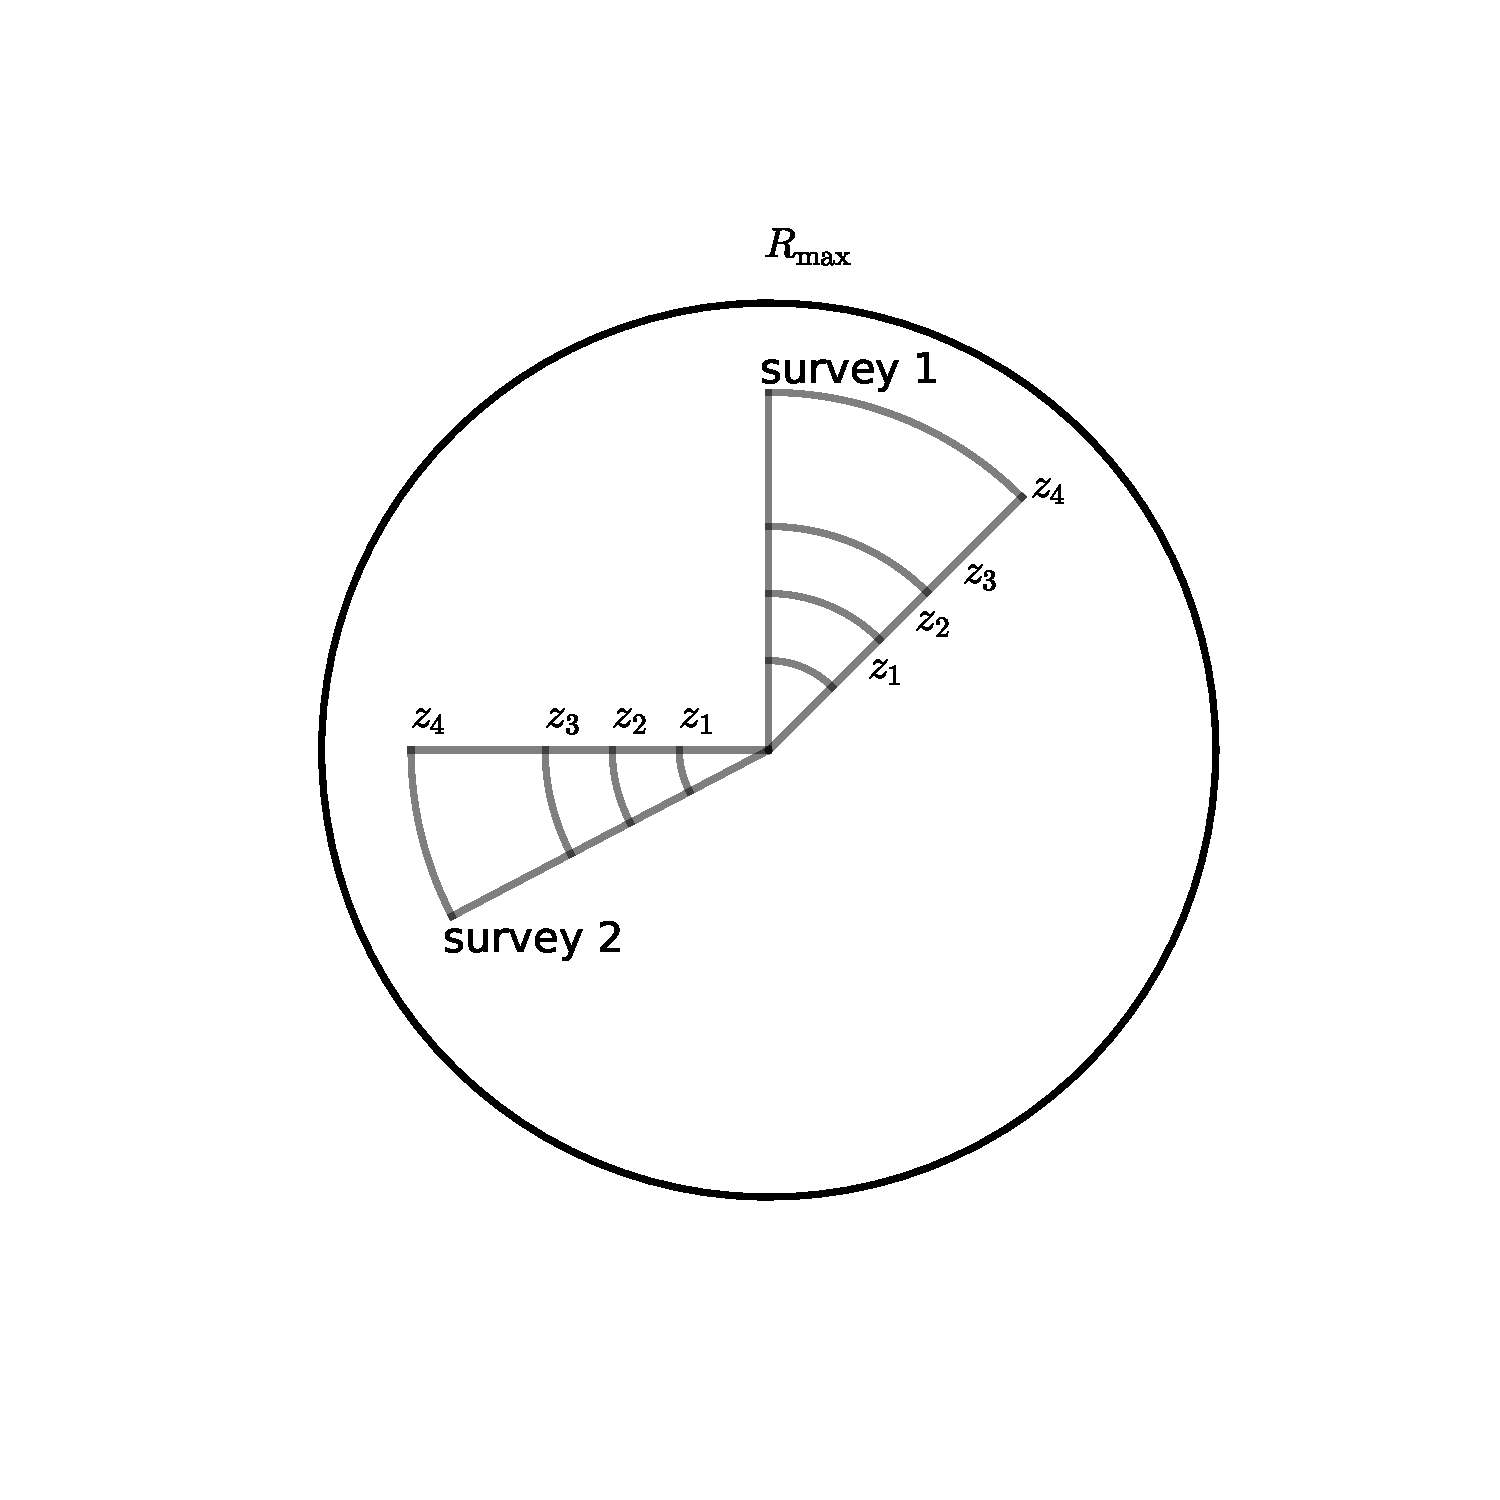
\includegraphics[width=1\textwidth]{field.pdf}
  \caption{Cartoon depiction of our basis definition scenario. The basis $\psi_\alpha$ is defined on a ball with an $R_\text{max}$ that exceeds the depth of any survey. Each $\bar{\delta}$ is calculated in a redshift slice of the a survey. }
\label{fig:field}
\end{figure}


 
\subsubsection{Covariance of super modes}
In our basis the super survey mode is defined as 
\begin{align} 
\begin{split} 
\delta_\alpha& = \int \delta(\mathbf{r}) \jl{\alpha}(k_\alpha r) \sph{\alpha}{r} d^3 \mathbf{r}  \\
& = \int \dk \delta(\mathbf{k}) \int_0^{R_\text{max}} dr^2 \jl{\alpha}(k_\alpha r) \int d^2 \hat{r} e^{ikr \hat{k} \cdot \hat{r}} \sph{\alpha}{r} \\
& =4 \pi i^{l_\alpha}\int  \dk \delta(\mathbf{k})  \sph{\alpha}{k}  \int_0^{R_\text{max}} dr^2 \jl{\alpha}(k_\alpha r) \jl{\alpha}(kr)  ~,
\end{split} 
\end{align} 
where in the second equality $\delta(\mathbf{r})=(2\pi)^{-3} \int d^3 \mathbf{k} \exp(i \mathbf{k} \cdot \mathbf{r}) \delta(\mathbf{k})$ was used and in the third equality the following identity was used 
\begin{align} \int_{S^2} d^2 \hat{r} \sph{\alpha}{r} e^{i \mathbf{k} \cdot \mathbf{r}} = 4 \pi i^{l_\alpha} j_{l_\alpha}(k r)\sph{\alpha}{k}~.
\end{align}
Including a normalization
\begin{align}\label{normalization}
N_\alpha&=\int{d^3\mathbf{r}\sph{\alpha}{r} \sph{\alpha}{r} j_\alpha(k_\alpha r) j_\alpha(k_\alpha r)} \\
&=  I_\alpha(k_\alpha, R_\text{max})  \int_\Omega \sph{\alpha}{r} \sph{\alpha}{r} \hat{r}\\
& =I_\alpha(k_\alpha, R_{\text{max}})  
\end{align}
where $ I_\alpha(k_\alpha, r_{\text{max}}) $ is as defined in \eqref{norm_final} and $ \int_\Omega \sph{\alpha}{r} \sph{\alpha}{r} \hat{r}=1$, we have
\begin{align} 
\delta_\alpha= \frac{4 \pi i^{l_\alpha}}{N_\alpha} \int  \dk \delta(\mathbf{k})  \sph{\alpha}{k}  \int_0^{R_\text{max}} dr^2 \jl{\alpha}(k_\alpha r) \jl{\alpha}(kr)  ~.
\end{align} 
To get the covariance of the super survey field we take the ensemble average:
\begin{align} 
\begin{split} 
\langle \delta_\alpha \delta_\beta \rangle &= \frac{ (4 \pi)^2}{N_\alpha N_\beta} \int  \dkv{1} \dkv{2} \langle \delta(\mathbf{k}_1) \delta^*(\mathbf{k}_2) \rangle \sph{\alpha}{k_1} \sph{\beta}{k_2} \\
& \;\;\; \times   \int_0^{R_\text{max}}  dr r^2 \jl{\alpha}(k_\alpha r) \jl{\alpha}( k_1 r) \int_0^{R_\text{max}}  dr r^2 \jl{\beta}(k_\beta r) \jl{\beta}( k_2 r)  \\
&= \frac{ (4 \pi)^2}{N_\alpha N_\beta} \int \dk P(k) I_\alpha(k, R_\text{max}) \times I_\beta(k, R_\text{max})\sph{\alpha}{k_1}Y^R_{l_\beta m_\beta}(-\hat{k_1})\\
&=\frac{2}{\pi N_\alpha N_\beta}\int{k^2 dk P(k) \delta_{l_\alpha,l_\beta}\delta_{m_\alpha,m_\beta} I_\alpha(k, R_\text{max}) \times I_\beta(k, R_\text{max})}~,
\end{split} 
\end{align} 
where $(2 \pi)^3 \delta^3_\text{D}( \mathbf{k} + \mathbf{k}') P(k) =  \langle \delta(\mathbf{k}) \delta^*(\mathbf{k}') \rangle$ was used along with the definition 
\begin{align} 
\begin{split} 
I_\alpha(k,  R_\text{max}) & =  \int_0^{R_\text{max}}dr r^2 \jl{\alpha}(k_\alpha r) \jl{\alpha}( k r) \\
& = \frac{\pi}{2} \sqrt{ \frac{1}{k _ \alpha k}} \int_0^{R_\text{max}}dr r J_{l_\alpha+ 1/2}(k_\alpha r)  J_{l_\alpha+ 1/2}( k r) \\
& = \frac{\pi}{2} \frac{ R_\text{max}}{ \sqrt{ k _ \alpha k}}\frac{\left[k_\alpha J_{l_\alpha+ 1/2}( k  R_\text{max})J_{l_\alpha+ 1/2}'(k_\alpha  R_\text{max}) - k J_{l_\alpha+ 1/2}(k_\alpha  R_\text{max})J_{l_\alpha+ 1/2}'(k  R_\text{max})\right]}{k^2 - k_\alpha^2}\\
& = \frac{\pi}{2} \frac{ R_\text{max}}{ \sqrt{ k _ \alpha k}}\frac{\left[k_\alpha J_{l_\alpha+ 1/2}( k  R_\text{max})J_{l_\alpha- 1/2}(k_\alpha  R_\text{max}) - k J_{l_\alpha+ 1/2}(k_\alpha  R_\text{max})J_{l_\alpha- 1/2}(k  R_\text{max})\right]}{k^2 - k_\alpha^2}\\
& = \frac{\pi}{2} \frac{ R_\text{max}}{ \sqrt{ k _ \alpha k}}\frac{k_\alpha J_{l_\alpha+ 1/2}( k  R_{\text{max}})J_{l_\alpha- 1/2}(k_\alpha  R_\text{max})}{k^2 - k_\alpha^2}~,
\end{split} 
\end{align}
where in the last step we have use $J_{l_\alpha+1/2}(k_\alpha R_\text{max})=0$, from the defining property of $k_\alpha$. In the special case $k=k_\alpha$, we can simplify $N_\alpha = I_\alpha(k,R_\text{max})$:

\begin{align}
N_\alpha = I_\alpha(k_\alpha,  R_\text{max}) & = \lim_{k\to k_\alpha} \frac{\pi}{2} \frac{ R_\text{max}}{ \sqrt{ k _ \alpha k}}\frac{k_\alpha J_{l_\alpha+ 1/2}( k  R_\text{max})J_{l_\alpha- 1/2}(k_\alpha  R_\text{max})}{k^2 - k_\alpha^2}\\
&=\lim_{k\to k_\alpha}\frac{\pi R_\text{max}}{2} \frac{J_{l_\alpha+ 1/2}( R_\text{max})J_{l_\alpha- 1/2}(k_\alpha  R_\text{max})}{k^2 - k_\alpha^2}\label{pre_lhopital}\\
&=\lim_{k\to k_\alpha}\frac{\pi R_\text{max}}{2} \frac{r_\text{max}J'_{l_\alpha+ 1/2}(k R_\text{max})J_{l_\alpha- 1/2}(k_\alpha  R_\text{max})}{2 k}\label{post_lhopital}\\
&=\lim_{k\to k_\alpha}\frac{\pi R_\text{max}^2}{2} \frac{\left[\frac{l_\alpha+1/2}{k R_{\text{max}}}J_{l_\alpha+1/2}(k R_\text{max})-J_{l_\alpha+3/2}(k_\alpha R_\text{max})\right]J_{l_\alpha- 1/2}(k_\alpha  R_\text{max})}{2 k}\label{post_recurrence}\\
&=-\frac{\pi r_\text{max}^2}{4 k_\alpha}J_{l_\alpha+3/2}(k_\alpha{R_\text{max}})J_{l_\alpha- 1/2}(k_\alpha  R_\text{max})\label{norm_final} ~,
\end{align}
where between \eqref{pre_lhopital} and \eqref{post_lhopital} we have used L'H$\hat{\text{o}}$pital's rule, and between \eqref{post_lhopital} and \eqref{post_recurrence} we have used a recurrence relation for the Bessel functions, $J'_n(x)=\frac{n}{x}J_n{x}-J_{n+1}(x)$.

%\end{document}  